\documentclass[conference]{IEEEtran}
\IEEEoverridecommandlockouts
% The preceding line is only needed to identify funding in the first footnote. If that is unneeded, please comment it out.
\usepackage{cite}
\usepackage{amsmath,amssymb,amsfonts}
\usepackage{algorithmic}
\usepackage{graphicx}
\usepackage{textcomp}
\usepackage{xcolor}

% Increase Size
\usepackage{amsmath}
\usepackage{relsize}

% Write Optimization problems
\usepackage{amsmath}
\DeclareMathOperator*{\Max}{Max}
\DeclareMathOperator*{\Min}{Min}
\usepackage{optidef}


\def\BibTeX{{\rm B\kern-.05em{\sc i\kern-.025em b}\kern-.08em
    T\kern-.1667em\lower.7ex\hbox{E}\kern-.125emX}}

\begin{document}

\title{Diversification of risk through portfolio investment\\
}

\makeatletter
    \newcommand{\linebreakand}{%
      \end{@IEEEauthorhalign}
      \hfill\mbox{}\par
      \mbox{}\hfill\begin{@IEEEauthorhalign}
    }
\makeatother

\author{

\IEEEauthorblockN{1\textsuperscript{st} Krishna Teja Chilukuri}
\IEEEauthorblockA{\textit{Mathematics and Computing} \\
\textit{Indian Institute of Technology, Hyderabad} \\
Hyderabad, India \\
ma20btech11005@iith.ac.in
}

\and

\IEEEauthorblockN{2\textsuperscript{nd} Sumanth NR}
\IEEEauthorblockA{\textit{Mathematics and Computing} \\
\textit{Indian Institute of Technology, Hyderabad} \\
Hyderabad, India \\
ma20btech11016@iith.ac.in
}

\linebreakand

\IEEEauthorblockN{3\textsuperscript{rd} Prajwaldeep Kamble}
\IEEEauthorblockA{\textit{Mathematics and Computing} \\
\textit{Indian Institute of Technology, Hyderabad} \\
Hyderabad, India \\
ma20btech11013@iith.ac.in
}

\and

\IEEEauthorblockN{4\textsuperscript{th} Karthik Kurugodu}
\IEEEauthorblockA{\textit{Mathematics and Computing} \\
\textit{Indian Institute of Technology, Hyderabad} \\
Hyderabad, India \\
ma20btech11008@iith.ac.in
}

\linebreakand

\IEEEauthorblockN{5\textsuperscript{th} Nikhil Kongara}
\IEEEauthorblockA{\textit{Mathematics and Computing} \\
\textit{Indian Institute of Technology, Hyderabad} \\
Hyderabad, India \\
ma20btech11011@iith.ac.in
}

% \and
% \IEEEauthorblockN{\textsuperscript{}}
% \IEEEauthorblockA{\textit{} \\
% \textit{}\\
% %  \\
% }
}

\maketitle


\begin{abstract}
Diversification of Risks through portfolio investments using Markowitz Model (Mean Variance Model).
\linebreak
Comparing Value at Risk(VaR) and Conditional Value at Risk(CVaR) using Monte Carlo Method
\end{abstract}

\begin{IEEEkeywords}
portfolio, risk, diversification, Markowitz model, VaR, CVaR, Monte Carlo
\end{IEEEkeywords}

\section{Introduction}
The stock exchange markets are characterized by high dynamics of the investment activity, mainly portfolio investments. The existing relation between yield and risk, on one side, and the portfolio diversification, on the other side, are two basic aspects allowing the investors to build up a portfolio founded on the yield and risk targets which they are aiming. 

In the first part, we will use Markowitz model to demonstrate that diversification of portfolio is better. In the second part, we will compare the VaR and CVaR risk measures using Monte Carlo method

\subsection{Portfolio}
    An investment portfolio is a collection of assets owned by an investor. This portfolio can include investment securities such as bonds, stocks, mutual funds, pension plans, real estate and even physical assets such as gold (coins or bars). Basically, this includes every asset that can grow in value or provide returns. Many even invest in valuable artefacts for future profits.
    
    % (Referred from https://www.edelweiss.in/investology/introduction-to-investing-c6eaf4/what-is-an-investment-portfolio-789abc)

\subsection{Portfolio management}
    Portfolio management involves building and overseeing a selection of investments that will meet the long-term financial goals and risk tolerance of an investor.
    
\subsection{Sharpe Ratio}
    Sharpe ratio measures the performance of an investment such as a security or portfolio compared to a risk-free asset, after adjusting for its risk. It is defined as the difference between the returns of the investment and the risk-free return, divided by the standard deviation of the investment returns. It represents the additional amount of return that an investor receives per unit of increase in risk.
    

\section{Markowitz Model}
The Markowitz model for diversifying the financial instruments portfolio may lead to the identification of some optimum portfolios of risky assets, respectively of portfolios providing a maximum of the estimated yield for a certain level of the risk which the capital investors are willing to undertake depending on their behaviour against the risk.

\subsection{Assumptions of Markowitz Model}
    \begin{itemize}
        \item Investors are rational (they seek to maximize returns while minimizing risk).
        \item Investors will accept increased risk only if compensated with higher expected returns.
        \item Investors receive all pertinent information regarding their investment decision in a timely manner.
    \end{itemize}

\subsection{Variables}
    \subsubsection{Expected Return for Portfolio}
        \[
            E_p = \sum_{i=1}^{n}
            w_i E(r_i)
        \]
    
    \subsubsection{Co variance}
        \[
            \sigma_{ij} = 
            \frac{1}{T-1}
            \sum_{t=1}^{T}
            (R_{i_{(t)}} - E(r_i)) (R_{j_{(t)}} - E(r_j))
        \]
        
        $ \textbf{where,} $
        \begin{itemize}
            \item $ T $ : Number of Time periods
            \item $ R_{i_{(t)}} $: the yield of the asset “i” at the moment “t”
            \item $ E(r_i) $ : the average yield of the asset “i”; 

        \end{itemize}
    
    \text{\n}
    
    \subsubsection{Portfolio Variance of two assets (x and y)}
        \[
            \sigma_p^2 = 
            w_x^2\sigma_x^2 + 
            w_y^2\sigma_y^2 + 
            2 w_x w_y \sigma_{xy}
        \]
        
    \subsubsection{Portfolio Variance of n assets}
        \[
            \sigma_p^2 = 
            \sum_{i=1}^{n}
            \sum_{j=1}^{n}
            w_i w_j \sigma_{ij}
        \]
        \text{\n}
        \[
            \sigma_p^2 = 
            W^T C W
            \hspace{1.35cm}
        \]
        
        $ \textbf{where,} $
        \begin{itemize}
            \item $E(r_i)$ is the Expected return of $i^{th}$ asset
            \item $n$ is the number of assets
            \item $w_i$ is the weight of $i^{th}$ asset
            \item $W$ \in \hspace{0.1cm} ${\rm I\!R}^n$ is the Weights Vector
            \item $C$ \in \hspace{0.1cm} ${\rm I\!R}^n$\times \hspace{0.1cm} ${\rm I\!R}^n$ is the Co variance Matrix
        \end{itemize}
    
    \text{\n}
    \subsubsection {Risk}
        \[
            Risk = \sigma_p 
        \]
    
        In Markowitz Model, $ \sigma_{p} $ is considered to be the risk 
        
        $\text{Portfolio Risk is influenced by:}$
        \begin{itemize}
            \item The individual risks of each asset included in the portfolio; 
            \item The weight of each asset in the portfolio structure;
            \item The covariance between the assets yields, considered two by two.
        \end{itemize}
    
\subsection{Problem Formulation}

    \subsubsection{Calculating Minimum Risk given Minimum Return}
        
        \begin{mini}|l|
    	  {}{\mathlarger{\sigma_p^2}}{}{}
    	  \addConstraint {\sum_{i=1}^n w_i} {= 1, \quad w_i \geq 0} {}
    	  \addConstraint {E_p} {\geq \text{minimum return}} {}
    	  \notag
        \end{mini}
        
    \subsubsection{Calculating Maximum Return given Maximum Risk}
        
        \begin{maxi}|l|
    	  {}{\mathlarger{E_p}}{}{}
    	  \addConstraint {\sum_{i=1}^n w_i} {= 1, \quad w_i \geq 0} {}
    	  \addConstraint {\sigma_p^2} {\leq \text{(maximum risk)}^2} {}
    	  \notag
        \end{maxi}


\section{The analysis of the return and risk}

\subsection{Comparing Maximum Return given Maximum allowed risk}
    \begin{figure}[htbp]
    \centerline{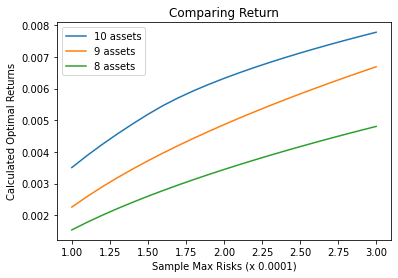
\includegraphics[scale=0.55]{graphs/return_vs_risk.png}}
    \caption{Optimal Return vs Max Risk allowed}
    \label{fig}
    \end{figure}
    We can clearly see that for the same amount of risk, investing higher number of assets gives us better returns
    
    \begin{figure}[htbp]
    \centerline{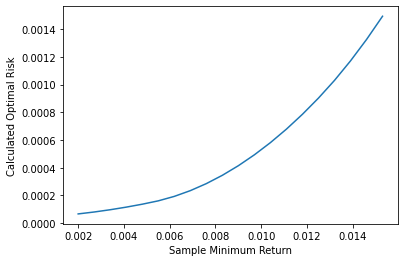
\includegraphics[scale=0.55]{graphs/risk_vs_return.png}}
    \caption{Minimum Risk vs Minimum Return}
    \label{fig}
    \end{figure}
    
    \begin{itemize}
        \item  We can infer that risk increases with return
        
        \item  We can also observe that the slope of the graph increases
    \end{itemize}
    

\section{Analysis}
From the graph, we can infer that for a given risk, optimal return increases with diversification

Therefore to invest in a portfolio, it is better to invest in more number of assets, i.e., diversifying the portfolio.

\pagebreak


\section{VaR and CVaR}

\subsection{Value at Risk (VaR)}
    Value-at-risk is \textbf{a statistical measure of the riskiness of financial entities or portfolios of assets}. It is defined as the maximum dollar amount expected to be lost over a given time horizon, at a pre-defined confidence level.
    
    Given a confidence level $\beta$ in [0, 1], the VaR of the portfolio at the confidence level $\beta$ is given by the smallest number “l” such that the probability that the loss “L” exceeds l is at most ($1-\beta$). Mathematically, if “L” is the loss of a portfolio, then VaRα(L) is the level $\beta$-quantile \\ 
    Drawbacks of VaR
    \begin{itemize}
        \item \textbf{Not subadditive}
        \item \textbf{Not convex}
    \end{itemize} 
    
    
\subsection{Conditional Value at Risk (CVaR)}
    Conditional Value at Risk (CVaR), also known as the expected shortfall, is a risk assessment measure that quantifies the amount of tail risk an investment portfolio has. CVaR is derived by taking a weighted average of the ``extreme" losses in the tail of the distribution of possible returns, beyond the value at risk (VaR) cutoff point.
    
\subsection{Methods to calculate VaR and CVaR}
    \begin{itemize}
        \item Historical method
        \item Variance-Covariance method 
        \item Monte Carlo simulation.
    \end{itemize}
    
    
    % \[ 
    %     \text{VaR}_{\alpha}(L) = \inf_{l \in \mathbb{R}} \left \{ \mathbb{P}(L \geq l) \geq 1 - \alpha \right \}
    % \]
    % If X is the return
    
% \subsection{Historic Method}
%     For a given time horizon $t$ and confidence level $\beta$ , the value at risk of a portfolio is the loss in the portfolio's market value over the time horizon $t$ that is exceeded with probability $1 - \beta$
%     \[ 
%         \text{VaR}_{\beta}(X) = \min_{t \in (0,T)} \left \{ X_{t} \in \mathbb{R}: F_{X}(X_{t}) \geq \beta \right \}
%     \]
%     \[
%         \text{CVaR}_{\beta}(X) = \text{VaR}_{\beta}(X) +
%         \frac{1}{\beta T} \sum_{t=1}^{T} \max(-X_{t} -
%         \text{VaR}_{\beta}(X), 0)
%     \]
    
% \textbf{where}, $X$ is the vector of random variables of dimension T, $X_i$ denoting the returns in the $i^{th}$ time period

\subsection{Mathematical Formulation}
    
    $\textbf{x} \in \mathbb{R}^n$ is the decision vector where n in the number of assets chosen from a certain subset $X$ of $\mathbb{R}^n$,
    
    $S \in \mathbb{R}^q$ is a vector of random variables denoting uncertainties (like Market Variables) that can affect the loss. 
    $S$ is assumed to have probability density of $p(S)$ for convenience.
    
    $f(\textbf{x}, S)$ is the loss associated with the portfolio. The distribution of f is induced by S.
    
    The probability of the loss not exceeding a threshold $\alpha$ is given by the cumulative distribution function, ($\alpha$ is the maximum risk allowed)
    \begin{equation}
        \Psi(\textbf{x}, \alpha) = 
        \underset{f(x, S) \leq \alpha}{\int}
        p(S) \, dS
    \end{equation}
    
    Let's say $\beta$ is the confidence level. VaR is the minimum value of $\alpha$ such that 
    $ \Psi(\textbf{x}, \alpha) \geq \beta $
    
    VaR associated with a portfolio $\mathbf{x}$, for a specified confidence level $\beta$ and time horizon t, is given by
    \begin{equation}
        \alpha_\beta(\textbf{x}) =
        \min \{ 
        \alpha \in \mathbb{R}: 
        \Psi(\textbf{x}, \alpha) \geq \beta
        \}
    \end{equation}
    
    Let's assume $ \Psi(\textbf{x}, \alpha) $ is smooth, CVaR is the conditional expectation of all the loss exceeding $\alpha_\beta(\textbf{x})$
    \begin{equation}
        \phi_\beta(\textbf{x}) = \mathbb{E}
        (f(\textbf{x}, S) \ | \ f(\textbf{x}, S) >  \alpha_\beta(\textbf{x}))
        \notag
    \end{equation}
    In can be expressed as
    \begin{equation}
        \phi_\beta(\textbf{x}) = 
        \frac{1}{1 - \beta} \
        \underset{f(\textbf{x}, S) \ \geq \ 
        \alpha_\beta(\textbf{x})} {\int}
        f(\textbf{x}, S) p(S) \, dS
    \end{equation}
    
    Rockafellar and Uryasev proposed an augmented function to characterize both 
    $\phi_\beta(\textbf{x})$ and 
    $\alpha_\beta(\textbf{x})$ as follow
    \begin{equation}
        F_\beta(\textbf{x}, \alpha) = 
        \alpha + \frac{1}{1 - \beta} \
        \underset{S \ \in \ \mathbb{R}^q} {\int}
        [f(\textbf{x}, S) - \alpha]^+ p(S) \, dS
    \end{equation}
    where 
    \[
        [z]^+ = 
        \begin{cases}
            z & \text{if} \ z > 0 \\
            0 & \text{if} \ z \leq 0
        \end{cases}
    \]
    
    The augmented function is Convex and continuously differentiable. Rockafellar and Uryasev proved that minimizing the augmented function is equivalent to solving for CVaR. \\ 
    
    Hence, 
    \begin{equation}
        \phi_\beta(\textbf{x}) = 
        \underset{\alpha \in \mathbb{R}} {\min}
        \ F_\beta(\textbf{x}, \alpha)
    \end{equation}
    
    Unlike equation (3), equation (5) does not require the VaR to be predetermined but is calculated as a part of the solution. \\
    
    The integral in equation (4) can be numerically approximated by Monte Carlo Approximation as
    
    \begin{equation}
        \overline{F}_\beta(\textbf{x}, \alpha) =
        \alpha + \frac{1}{q(1-\beta)} \ 
        \sum_{i=1}^q [f(\textbf{x}, S^i) - \alpha]^+
    \end{equation}


\section{Monte Carlo}

Monte Carlo simulations are used to model the probability of different outcomes in a process that cannot easily be predicted due to the intervention of random variables. It is a technique used to understand the impact of risk and uncertainty in prediction and forecasting models.

A Monte Carlo simulation can be used to tackle a range of problems in virtually every field such as finance, engineering, supply chain, and science. It is also referred to as a multiple probability simulation.

\subsection{Monte Carlo Simulation Method}
    A Monte Carlo simulation takes the variable that has uncertainty and assigns it a random value. The model is then run and a result is provided. This process is repeated again and again while assigning the variable in question with many different values. Once the simulation is complete, the results are averaged together to provide an estimate.
    
Here, we apply Monte Carlo Simulations on k random weights and find CVaR and VaR for each of them using 1000 simulations of their returns for next 10 days. \

\begin{figure}[htbp]
    \centerline{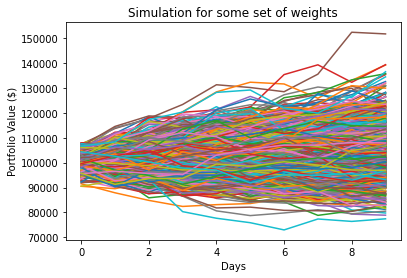
\includegraphics[scale=0.55]{graphs/simulation01.png}}
    \caption{Monte Carlo Simulation for some random set of weights}
    \label{fig}
\end{figure}

\begin{figure}[htbp]
    \centerline{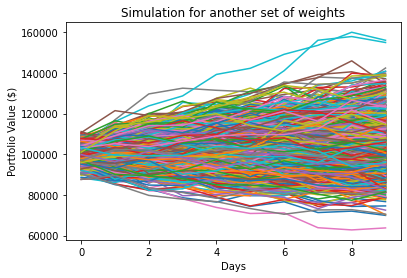
\includegraphics[scale=0.55]{graphs/simulation02.png}}
    \caption{Monte Carlo Simulation for another random set of weights}
    \label{fig}
\end{figure}


    
\section{Comaparing VaR and CVaR}

After simulating for around 800 random weights, for each weight, running 1000 Monte Carlo simulations, we calculate the VaR and CVaR for each weight.

We then compare VaR and CVaR for these 800 random weights

\pagebreak

\begin{figure}[htbp]
    \centerline{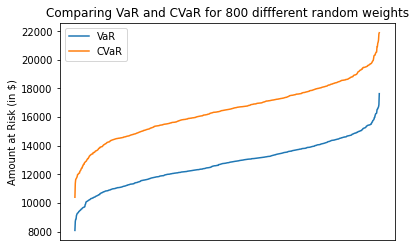
\includegraphics[scale=0.55]{graphs/comparing_VaR_CVaR.png}}
    \caption{Comparing VaR and CVaR}
    \label{fig}
\end{figure}



\section{Conclusions}

From the figure we can see that CVaR is always greater than VaR. So, for a risk averse investor it always better to optimize CVaR instead of VaR.

From the Mathematical Formulation, it can be observed that CVaR is a Convex Function and hence can be solved using the Convex Optimization techneques.

Also, CVaR is sub-additive while VaR is not which makes it a more easier function to deal with since sub-additivy is closely related to convexity. 

We thus conclude by stating that CVaR is a better form of risk measure than VaR. 

% \begin{figure}[htbp]
%     \centerline{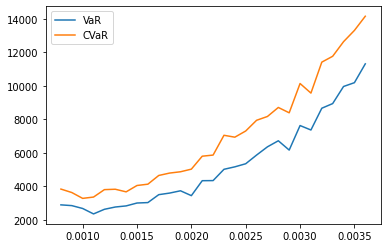
\includegraphics[scale=0.55]{graphs/fig2.png}}
%     \caption{VaR vs CVaR}
%     \label{fig}
% \end{figure}


% \section*{Acknowledgment}

% The preferred spelling of the word ``acknowledgment'' in America is without 
% an ``e'' after the ``g''. Avoid the stilted expression ``one of us (R. B. 
% G.) thanks $\ldots$''. Instead, try ``R. B. G. thanks$\ldots$''. Put sponsor 
% acknowledgments in the unnumbered footnote on the first page.

\begin{thebibliography}{00}
    \bibitem{b1} Johnny Chow ``Robustness of data-driven CVaR optimization using smoothing technique'' Waterloo, Ontario, Canada - 2014, pp. 2--6.
    \bibitem{b2} K.Nagarajan, J. Prabhakaran, Prediction of Stock Price Movements using Monte Carlo Simulation, in International Journal of Innovative Technology and Exploring Engineering (IJITEE) ISSN: 2278-3075, Volume-8 Issue-12, October 2019
    \bibitem{b3} Gabriela Victoria ANGHELACHE and Constantin ANGHELACHE, Diversifying the risk through portfolio investment in Theoretical and Applied Economics, Volume XXI (2014), No. 9(598), pp. 7-22 .
\end{thebibliography}
\vspace{12pt}


\end{document}
